%% sudo yum install tetex
%% sudo yum install texlive-elsarticle.noarch  texlive-sttools.noarch texlive-lipsum.noarch
%% pdflatex Machine_learning.tex && bibtex Machine_learning.aux && pdflatex Machine_learning.tex && pdflatex Machine_learning.tex


%\documentclass[a4paper,12pt]{}
\documentclass[final, paper=letter,5p,times,twocolumn]{elsarticle}
%\documentclass[preprint,review,8pt,times]{elsarticle}


%% or use the graphicx package for more complicated commands
%\usepackage{changebar}
\usepackage{graphicx}
\usepackage{caption}
\usepackage{subcaption}
\usepackage{multirow}
%% or use the epsfig package if you prefer to use the old commands
%% \usepackage{epsfig}

%% The amssymb package provides various useful mathematical symbols
\usepackage{tikz}
\usepackage{amsmath,amsfonts,amsthm,multicol,bm,lipsum} % Math packages
\usepackage{cuted}
%\usepackage{dsfont} % mathds{1}
%\usepackage{widetext} % 
\usepackage{listings}
\usepackage{amssymb}
\usepackage{hyperref}
%
%\usepackage[]{algorithm2e}
%% Macro
\newcommand{\ToDo}[1]{ToDo: \textbf{\textit{#1}}}
\newcommand{\CA}{computational anatomy}
%
\newdefinition{definition}{Definition}%
\newtheorem{theorem}{Theorem}%
\newtheorem{corollary}{Corollary}[theorem]
\newtheorem{lemma}[theorem]{Lemma}
%\newproposition{proposition}{Proposition}%
%\newlemma{lemma}{Lemma}%
%\AtEndEnvironment{theorem}{\null\hfill\qedsymbol}%

\begin{document}
%%%%%%%%%%%%%%%%%%%%%%%%%%%%%%%%%%%%%%%%%%%%%%%%%%%%%%%%%%%%%%%%%%%%%%%%%%
%%%%%%%%%%%%%%%%%%%%%%%%%%%%%%%%%%%%%%%%%%%%%%%%%%%%%%%%%%%%%%%%%%%%%%%%%%
%%%%%%%%%%%%%%%%%%%%%%%%%%%%%%%%%%%%%%%%%%%%%%%%%%%%%%%%%%%%%%%%%%%%%%%%%%
%%%%%%%%%%%%%%%%%%%%%%%%%%%%%%%%%%%%%%%%%%%%%%%%%%%%%%%%%%%%%%%%%%%%%%%%%%
\begin{frontmatter}

\title{Neural network}

\author[label1]{Yann Cobigo\corref{cor1}}
\address[label1]{University of California, San Francisco | ucsf.edu}
%\address[label2]{Address Two\fnref{label4}}

%\cortext[cor1]{I am corresponding author}
%\fntext[label3]{I also want to inform about\ldots}
%\fntext[label4]{Small city}

\ead{yann.cobigo@ucsf.edu}
\ead[url]{https://github.com/YannCobigo}

%% \author[label5]{Author Two}
%% \address[label5]{Some University}
%% \ead{author.two@mail.com}
%% 
%% \author[label1,label5]{Author Three}
%% \ead{author.three@mail.com}

\begin{abstract}
 \lipsum[11-15]
\end{abstract}

\begin{keyword}
%% keywords here, in the form: keyword \sep keyword
Fijee \sep electrode \sep PEM \sep CEM
%% MSC codes here, in the form: \MSC code \sep code
%% or \MSC[2008] code \sep code (2000 is the default)
\end{keyword}

\end{frontmatter}

%%%%%%%%%%%%%%%%%%%%%%%%%%%%%%%%%%%%%%%%%%%%%%%%%%%%%%%%%%%%%%%%%%%%%%%%%%
%%%%%%%%%%%%%%%%%%%%%%%%%%%%%%%%%%%%%%%%%%%%%%%%%%%%%%%%%%%%%%%%%%%%%%%%%%
%%%%%%%%%%%%%%%%%%%%%%%%%%%%%%%%%%%%%%%%%%%%%%%%%%%%%%%%%%%%%%%%%%%%%%%%%%
%%%%%%%%%%%%%%%%%%%%%%%%%%%%%%%%%%%%%%%%%%%%%%%%%%%%%%%%%%%%%%%%%%%%%%%%%%

\section{Introduction}

\lipsum[100-104]


%%%%%%%%%%%%%%%%%%%%%%%%%%%%%%%%%%%%%%%%%%%%%%%%%%%%%%%%%%%%%%%%%%%%%%%%%%
%%%%%%%%%%%%%%%%%%%%%%%%%%%%%%%%%%%%%%%%%%%%%%%%%%%%%%%%%%%%%%%%%%%%%%%%%%
\section{Decision tree}

A key property of tree-based models, which makes them popular in fields such as medical diagnosis, for example, is that they are readily interpretable by humans because they correspond to a sequence of binary decisions applied to the individual input variables. For instance, to predict a patient's disease, we might first ask ``is their temperature greater than some threshold?''. If the answer is yes, then we might next ask ``is their blood pressure less than some threshold?''. Each leaf of the tree is then associated with a specific diagnosis. \\

\subsection{Regression-type problems}

Regression-type problems are generally those where we attempt to predict the values of a continuous variable from one or more continuous and/or categorical predictor variables. For example, we may want to predict the selling prices of single family homes (a continuous dependent variable) from various other continuous predictors (e.g., square footage) as well as categorical predictors (e.g., style of home, such as ranch, two-story, etc.; zip code or telephone area code where the property is located, etc.; note that this latter variable would be categorical in nature, even though it would contain numeric values or codes).\\
If we used simple multiple regression, or some general linear model (GLM) to predict the selling prices of single family homes, we would determine a linear equation for these variables that can be used to compute predicted selling prices. There are many different analytic procedures for fitting linear models (GLM, GRM, Regression), various types of nonlinear models (e.g., Generalized Linear/Nonlinear Models (GLZ), Generalized Additive Models (GAM), etc.), or completely custom-defined nonlinear models (see Nonlinear Estimation), where we can type in an arbitrary equation containing parameters to be estimated. CHAID also analyzes regression-type problems, and produces results that are similar (in nature) to those computed by CART. Note that various neural network architectures are also applicable to solve regression-type problems.

\subsection{Classification-type problems}

Classification-type problems are generally those where we attempt to predict values of a categorical dependent variable (class, group membership, etc.) from one or more continuous and/or categorical predictor variables. For example, we may be interested in predicting who will or will not convert into AD, FTLD. These would be examples of simple binary classification problems, where the categorical dependent variable can only assume two distinct and mutually exclusive values. \\
In other cases, we might be interested in predicting which one of multiple different alternative consumer products (e.g., makes of cars) a person decides to purchase, or which type of failure occurs with different types of engines. In those cases there are multiple categories or classes for the categorical dependent variable. There are a number of methods for analyzing classification-type problems and to compute predicted classifications, either from simple continuous predictors (e.g., binomial or multinomial logit regression in GLZ), from categorical predictors (e.g., Log-Linear analysis of multi-way frequency tables), or both (e.g., via ANCOVA-like designs in GLZ or GDA). The CHAID also analyzes classification-type problems, and produces results that are similar (in nature) to those computed by CART. Note that various neural network architectures are also applicable to solve classification-type problems.




%%%%%%%%%%%%%%%%%%%%%%%%%%%%%%%%%%%%%%%%%%%%%%%%%%%%%%%%%%%%%%%%%%%%%%%%%%
\subsection{Growing the classification tree}

Growing a decision tree is a recursive process that can be done with several types of cost functions. The cost functions tend to minimize the fraction of points that were miss classified. In the Fig.~\ref{fig:DT_space_cuboid} we have two parameters $x = (\theta_{1}, \theta_{2})^{T}$, 31 AD subjects and 23 controles $n$ other type whose response are noted $y \in \{$~{\bf\textcolor{red}{x}},~{\bf\textcolor{green}{o}},~{\bf\textcolor{magenta}{*}},~$\cdots\}$.

There are various simple, but widely used, models that work by partitioning the input space into cuboid regions, whose edges are aligned with the axes, and then assigning a simple model (for example, a constant) to each region.  The process of selecting a specific model, given a new input $x$, can be described by a sequential decision making process corresponding to the traversal of a binary tree (one that splits into two branches at each node). Here we focus on a particular tree-based framework called classification and regression trees, or CART (Breiman et al., 1984), although there are many other variants going by such names as ID3 and C4.5 (Quinlan, 1986; Quinlan, 1993). \\

Fig.~\ref{fig:DT_space_cuboid} shows an illustration of a recursive binary partitioning of the input space, along with the corresponding tree structure Fig.~\ref{fig:DT_binary_tree}. In this example, the first step divides the whole of the input space into two regions according to whether $x_{1} \le \theta_{1}$ or $x_{1} > \theta_{1}$ where $\theta_{1}$ is a parameter of the model. This creates two subregions, each of which can then be subdivided independently. For instance, the region $x_{1} \le \theta_{1}$ is further subdivided according to whether $x_{2} \le \theta_{2}$ or $x_{2} \le \theta_{2}$ , giving rise to the regions denoted $A$ and $B$.\\
The recursive subdivision can be described by the traversal of the binary tree shown in Fig.~\ref{fig:DT_binary_tree}. For any new input $x$, we determine which region it falls into by starting at the top of the tree at the root node and following a path down to a specific leaf node according to the decision criteria at each node.

\begin{figure}[htbp]
   \begin{center}
      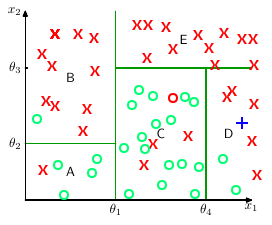
\includegraphics[scale=0.5, angle=0]{images/Decision_tree_space_cuboid_modified.png}
   \end{center}
   \caption{Partitioning of the space into cuboid. the symbole {\bf\textcolor{red}{x}} represents subjects with AD, symbole {\bf\textcolor{green}{o}} represents controls, and {\bf\textcolor{blue}{+}} represents an new point to classify.}
  \label{fig:DT_space_cuboid} 
\end{figure}

\begin{figure}[htbp]
   \begin{center}
      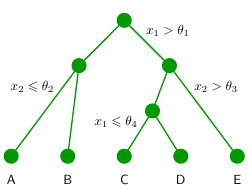
\includegraphics[scale=0.5, angle=0]{images/Decision_tree_binary_tree.png}
   \end{center}
   \caption{Binary tree result of the partitioning.}
  \label{fig:DT_binary_tree} 
\end{figure}

The decision process can be softened by moving to a probabilistic framework for combining models, as discussed in Section 14.5. For example, if we have a set of $K$ models for a conditional distribution $p(t|\bm{x}, k)$ where $x$ is the input variable, $t$ is the target variable, and $k = 1, \dots , K$ indexes the model, then we can form a probabilistic mixture of the form

$$
p(t|\bm{x}) = \sum_{k=1}^{K} \pi_{k}(\bm{x})p(t|\bm{x},k)
$$

in which $ \pi_{k} = p(k|\bm{x})$ represent the input-dependent mixing coefficients. Such models can be viewed as mixture distributions in which the component densities, as well as the mixing coefficients, are conditioned on the input variables and are known as mixtures of experts. 

\paragraph{Greedy optimization}{A greedy optimization is generally done by starting with a single root node, corresponding to the whole input space, and then growing the tree by adding nodes one at a time. At each step there will be some number of candidate regions in input space that can be split, corresponding to the addition of a pair of leaf nodes to the existing tree. For each of these, there is a choice of which of the $D$ input variables to split, as well as the value of the threshold. The joint optimization of the choice of region to split, and the choice of input variable and threshold, can be done efficiently by exhaustive search noting that, for a given choice of split variable and threshold, the optimal choice of predictive variable is given by the local average of the data for the regression, as noted earlier. This is repeated for all possible choices of variable to be split, and the one that gives the smallest residual sum-of-squares error is retained.
Given a greedy strategy for growing the tree, there remains the issue of when to stop adding nodes. A simple approach would be to stop when the reduction in residual error falls below some threshold. However, it is found empirically that often none of the available splits produces a significant reduction in error, and yet after several more splits a substantial error reduction is found. For this reason, it is com- mon practice to grow a large tree, using a stopping criterion based on the number of data points associated with the leaf nodes, and then prune back the resulting tree.}

\paragraph{Sub-optimization}{One limitation of decision trees is that the division of input space is based on hard splits in which only one explenatory variable is responsible for making predictions for any given value of the input variables, Fig.~\ref{fig:DT_space_cuboid},\ref{fig:DT_binary_tree}. It can make the global optimization sub-optimal, since the optimal decision on the first node, does not imply the rest of the nodes will split the best way. In other words, the first node impose a constraint. }

\begin{itemize}
\item Majority of votes: In the region $R$, the cost function $\mathcal{L} = \underset{y}{\min} \frac{1}{N_{R}}\sum_{i} I(y_{i} \ne y)$. Example, If we select the area $D$ from the Fig.~\ref{fig:DT_space_cuboid}, $N_{R} = 7$, and $\mathcal{L}_{D} = \underset{y}{\min} \{ \frac{5}{7}^{(o)}, \frac{2}{7}^{(x)}\} = \frac{2}{7}$, the response selected is {\bf\textcolor{red}{x}}.
\item Entropy: In the region $R$, we minimize the entropy $\mathcal{H}_{R} = - \sum_{y} p(y)\ln p(y)$. Following the same example: $\mathcal{H}_{D} = -\frac{5}{7}\ln(\frac{5}{7}) - \frac{2}{7}\ln(\frac{2}{7}) = (0.24)^{(x)} + (0.36)^{(o)} = 0.60$. The response selected is {\bf\textcolor{red}{x}}. Another advange of the entropy is its continuous form allowing the replacement of a griddy algorithm with a gradient descent.
  \item sum-of-squares (smallest residual), Gini index, \dots Also autorize the gradient descent.
\end{itemize}

Consider the regression problem in which the goal is to predict a single target variable $t$ from a $D$-dimensional vector $x = (x_{1}, \dots , x_{D})^{T}$ of input variables. The training data consists of input vectors $\{x_{1} , \dots , x_{N} \}$ along with the corresponding continuous labels $\{t_{1} , \dots , t_{N} \}$. If the partitioning of the input space is given, and we minimize the sum-of-squares error function, then the optimal value of the predictive variable within any given region is just given by the average of the values of $t_{n}$ for  those data points that fall in that region.


\subsubsection{Classification-type: Data on Children who have had Corrective Spinal Surgery}

Let's use the data frame kyphosis to predict a type of deformation (kyphosis) after surgery, from age in months (Age), number of vertebrae involved (Number), and the highest vertebrae operated on (Start). The statistics is presented Tab.~\ref{tab:Kyphosis}. The decision tree for Kyphosis is represented Fig.~\ref{fig:Tree_for_Kyphosis}.

\paragraph{Data set}{
  \begin{itemize}
  \item Description: The kyphosis data frame has 81 rows and 4 columns. representing data on children who have had corrective spinal surgery
  \item Format: This data frame contains the following columns:
    \begin{itemize}
    \item Kyphosis: a factor with levels absent present indicating if a kyphosis (a type of deformation) was present after the operation.
    \item Age: in months
    \item Number: the number of vertebrae involved
    \item Start: the number of the first (topmost) vertebra operated on.
    \end{itemize}
  \item Source: John M. Chambers and Trevor J. Hastie eds. (1992) Statistical Models in S, Wadsworth and Brooks/Cole, Pacific Grove, CA.
  \end{itemize}
}

\begin{table}[]
\begin{tabular}{cccc}
  Kyphosis   &    Age           &       Number    &       Start    \\
  absent :64 &  Min.   :  1.00  &  Min.   : 2.000 &  Min.   : 1.00  \\
  present:17 &  1st Qu.: 26.00  &  1st Qu.: 3.000 &  1st Qu.: 9.00  \\
             & Median : 87.00   &  Median : 4.000 &  Median :13.00  \\
             & Mean   : 83.65   &  Mean   : 4.049 &  Mean   :11.49  \\
             & 3rd Qu.:130.00   &  3rd Qu.: 5.000 &  3rd Qu.:16.00  \\
             & Max.   :206.00   &  Max.   :10.000 &  Max.   :18.00
\end{tabular}
\label{tab:Kyphosis}
\caption{Statistics on Children who have had Corrective Spinal Surgery}
\end{table}

\begin{figure}[htbp]
   \begin{center}
      \includegraphics[scale=0.35, angle=-90]{images/Classification_Tree_for_Kyphosis.png}
   \end{center}
   \caption{Classification Tree for Kyphosis.}
  \label{fig:Tree_for_Kyphosis} 
\end{figure}

\subsubsection{Regression-type: Data Automobile Data From 'Consumer Reports' 1990}

In this example we will predict car mileage from price, country, reliability, and car type. The \texttt{cu.summary} data frame has 117 rows and 5 columns, giving data on makes of cars taken from the April, 1990 issue of Consumer Reports. The statistics is presented Tab.~\ref{tab:cu.summary}. The regression tree is represented on the Fig.~\ref{fig:Tree_for_Kyphosis}.

\paragraph{Data set}{
  \begin{itemize}
  \item Price: a numeric vector giving the list price in US dollars of a standard model
  \item Country: of origin, a factor with levels Brazil, England, France, Germany, Japan, Japan/USA, Korea, Mexico, Sweden and USA
  \item Reliability: an ordered factor with levels Much worse < worse < average < better < Much better
  \item Mileage: fuel consumption miles per US gallon, as tested.
  \item Type:a factor with levels Compact Large Medium Small Sporty Van
  \end{itemize}
}

\begin{center}
\begin{table*}[ht]
\begin{tabular}{ccccc}
     Price     &       Country &       Reliability &   Mileage    &       Type   \\
 Min.   : 5866 &  USA      :49 &  Much worse :18   & Min.   :18.00 &  Compact:22  \\
 1st Qu.:10125 &  Japan    :31 &  worse      :12   & 1st Qu.:21.00 &  Large  : 7  \\
 Median :13150 &  Germany  :11 &  average    :26   & Median :23.00 &  Medium :30  \\
 Mean   :15743 &  Japan/USA: 9 &  better     : 8   & Mean   :24.58 &  Small  :22  \\
 3rd Qu.:18900 &  Korea    : 5 &  Much better:21   & 3rd Qu.:27.00 &  Sporty :26  \\
 Max.   :41990 &  Sweden   : 5 &  NA's       :32   & Max.   :37.00 &  Van    :10  \\
\end{tabular}
\label{tab:cu.summary}
\caption{Statistics on Automobile Data From 'Consumer Reports' 1990}
\end{table*}
\end{center}

\begin{figure}[htbp]
   \begin{center}
      \includegraphics[scale=0.35, angle=-90]{images/Regression_Tree_for_Mileage.png}
   \end{center}
   \caption{Regression Tree for Mileage.}
  \label{fig:Tree_for_Kyphosis} 
\end{figure}

\subsection{Random forest}

Simple method, state of the art in classification (Carvana, 2006).
Random forests improve predictive accuracy by generating a large number of bootstrapped trees (based on random samples of variables), classifying a case using each tree in this new "forest", and deciding a final predicted outcome by combining the results across all of the trees (an average in regression, a majority vote in classification).

\subsubsection{Boostrap aggregation, {\it a.k.a.} bagging (Breiman, 1996)}

Bootstrap Aggregation is a general procedure that can be used to reduce the variance for those algorithm that have high variance. An algorithm that has high variance are decision trees, like classification and regression trees (CART). When bagging with decision trees, we are less concerned about individual trees overfitting the training data. For this reason and for efficiency, the individual decision trees are grown deep (e.g. few training samples at each leaf-node of the tree) and the trees are not pruned. These trees will have both high variance and low bias. These are important characterize of sub-models when combining predictions using bagging. The only parameters when bagging decision trees is the number of samples and hence the number of trees to include. This can be chosen by increasing the number of trees on run after run until the accuracy begins to stop showing improvement (e.g. on a cross validation test harness). Just like the decision trees themselves, Bagging can be used for classification and regression problems. \\

When we trained multiple polynomials fitting data simulated around a sinusoid with noise, and then averaged the resulting functions, the contribution arising from the variance term tended to cancel, leading to improved predictions. When we averaged a set of low-bias models (corresponding to higher order polynomials), we obtained accurate predictions for the underlying sinusoidal function from which the data were generated.\\

In practice, of course, we have only a single data set, and so we have to find a way to introduce variability between the different models within the committee. One approach is to use bootstrap data sets. Consider a regression problem in which we are trying to predict the value of a single continuous variable, and suppose we generate $M$ bootstrap data sets and then use each to train a separate copy $y_{m}(\bm{x})$ of a predictive model where $m = 1, \dots , M$. The committee prediction is given by

$$
y_{commity}(\bm{x}) = \frac{1}{M} \sum_{m = 1}^{M} y(\bm{x})
$$

\begin{itemize}
\item Create many (e.g. 100) random sub-samples of our dataset with replacement.
\item Train a CART model on each sample.
\item Given a new dataset, calculate the average prediction from each model.
\end{itemize}

\subsubsection{Bagging to random forest (Breiman, 19XX)}

Random Forests are an improvement over bagged decision trees. A problem with decision trees like CART is that they are greedy. They choose which variable to split on using a greedy algorithm that minimizes error. As such, even with Bagging, the decision trees can have a lot of structural similarities and in turn have high correlation in their predictions. Combining predictions from multiple models in ensembles works better if the predictions from the sub-models are uncorrelated or at best weakly correlated.  \\
Random forest changes the algorithm for the way that the sub-trees are learned so that the resulting predictions from all of the subtrees have less correlation. It is a simple tweak. In CART, when selecting a split point, the learning algorithm is allowed to look through all variables and all variable values in order to select the most optimal split-point. The random forest algorithm changes this procedure so that the learning algorithm is limited to a random sample of features of which to search. The number of features that can be searched at each split point $m$ must be specified as a parameter to the algorithm. You can try different values and tune it using cross validation.

\begin{itemize}
\item For classification a good default is: $m = \sqrt{d}$
\item For regression a good default is: $m = d/3$
\end{itemize}

Where $m$ is the number of randomly selected features that can be searched at a split point and $d$ is the number of dimensions. For example, if a dataset had 25 dimensions for a classification problem, then:

\begin{itemize}
\item $m = \sqrt{25}$
\item $m = 8$
\end{itemize}

\subsubsection{Accuracy}

For each bootstrap sample taken from the training data, there will be samples left behind that were not included. These samples are called Out-Of-Bag samples or OOB. The performance of each model on its left out samples when averaged can provide an estimated accuracy of the bagged models. This estimated performance is often called the OOB estimate of performance. These performance measures are reliable test error estimate and correlate well with cross validation estimates.

\subsubsection{Classification-type: Kyphosis example with random forest}

\begin{itemize}
\item Call:  randomForest(formula = Kyphosis \~ Age + Number + Start, data = kyphosis) 
\item Type of random forest: classification
\item Number of trees: 500
\item No. of variables tried at each split: 1
\item OOB estimate of  error rate: 19.75\%
\end{itemize}

\begin{table}[]
\begin{tabular}{cccc}
          & absent & present & class.error \\
absent    &   60   &     4   & 0.0625000 \\
present   &   12   &     5   & 0.7058824 \\
\end{tabular}
\caption{Confusion matrix.}
\end{table}

%%%%%%%%%%%%%%%%%%%%%%%%%%%%%%%%%%%%%%%%%%%%%%%%%%%%%%%%%%%%%%%%%%%%%%%%%%
%%%%%%%%%%%%%%%%%%%%%%%%%%%%%%%%%%%%%%%%%%%%%%%%%%%%%%%%%%%%%%%%%%%%%%%%%%
\section{Conclusion}

\lipsum[6-10]

\section*{References}
%% References with bibTeX database:
\bibliographystyle{Bibliography/elsarticle-num}

\bibliography{Bibliography/sample}


\end{document}
